\chapter{Results and Discussions}

The performance of the Visual Inspection of Solar Farm system is evaluated through experimental observations and analytical interpretation. The results demonstrate the effectiveness of the system in detecting solar panel defects and generating inspection reports for maintenance planning. This chapter presents the experimental results obtained from the trained deep learning model, followed by a detailed discussion of system performance, comparisons, and insights derived from the observations.

\section{Experimental Results}

The system was tested using RGB images collected from solar panel installations under different environmental conditions. The objective was to evaluate the ability of the system to detect common faults such as dust accumulation, bird droppings, physical damage, electrical damage, and snow coverage.

\begin{figure}[H]
\centering
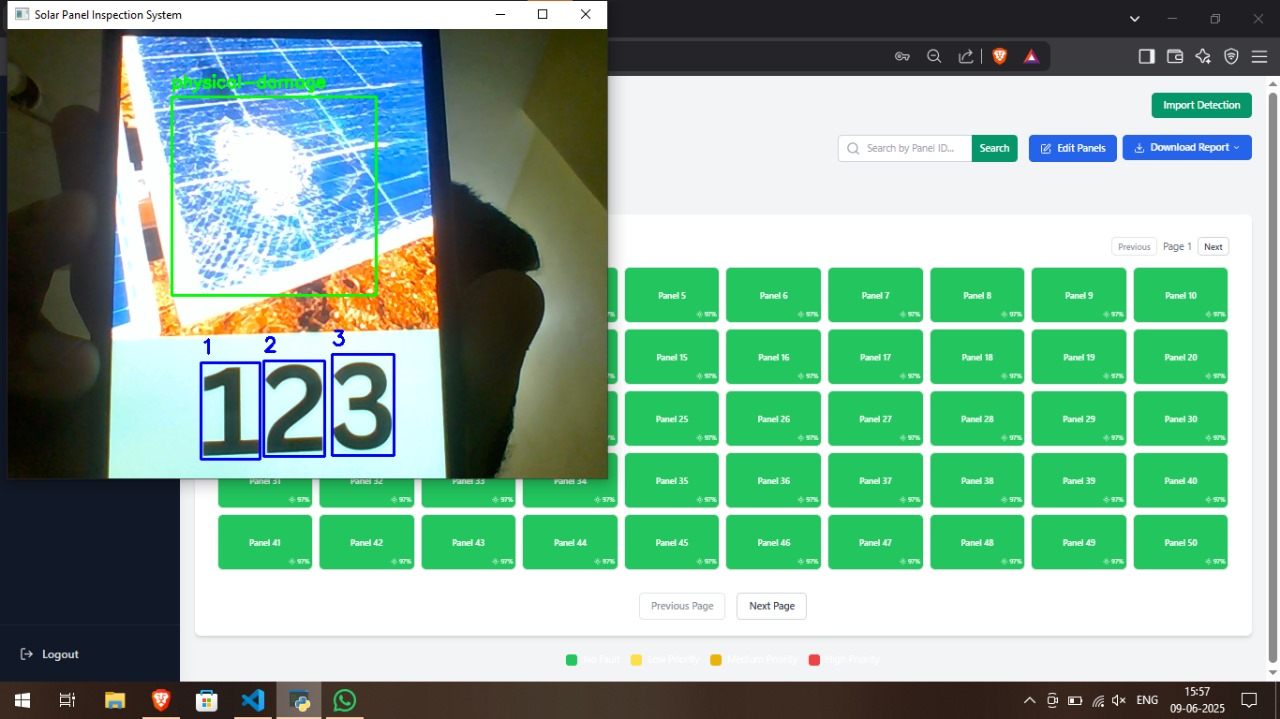
\includegraphics[width=0.75\textwidth]{figure/5.1.jpeg}
\caption{Live detection of faults}
\label{fig:hardwareprototype}
\end{figure}

Fig.~\ref{fig:hardwareprototype} shows sample inference results generated by the trained YOLO model. The model successfully detects and classifies multiple categories of solar panel defects by drawing bounding boxes around affected regions.

During testing, the system successfully processed solar panel images collected under varying operating conditions. The RGB image analysis module was capable of identifying multiple fault categories with satisfactory accuracy and consistency.

The deep learning-based fault detection model achieved promising performance in identifying defects across different inspection scenarios. The trained model demonstrated effective localization and classification capabilities, thereby reducing the need for manual inspection.

The monitoring dashboard successfully displayed inspection results, detected defect categories, and maintenance recommendations in real time, enabling operators to quickly assess the condition of the solar farm.

\begin{figure}[H]
\centering
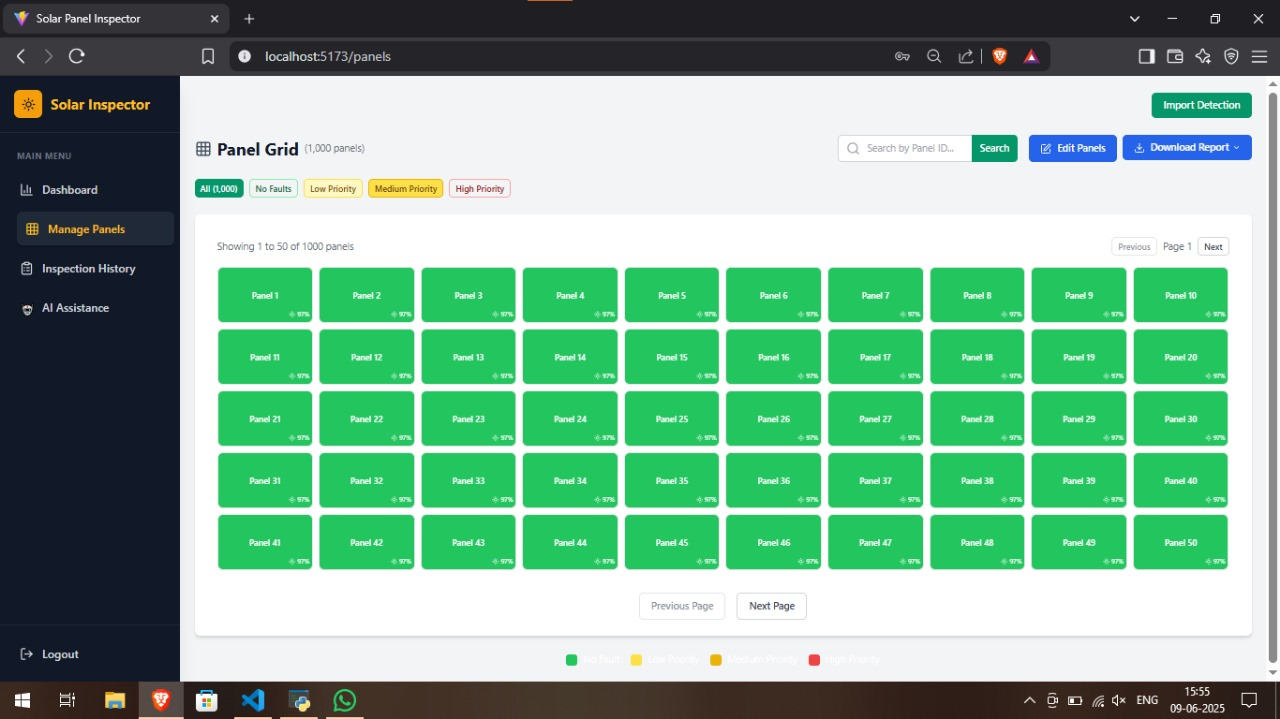
\includegraphics[width=0.75\textwidth]{figure/5.2.jpeg}
\caption{Monitoring dashboard displaying detected faults and inspection reports}
\label{fig:webalert}
\end{figure}

As shown in Fig.~\ref{fig:webalert}, the dashboard provides a centralized interface for visualizing detected faults, prediction confidence values, and inspection summaries. This assists maintenance personnel in decision-making and planning corrective actions.

\section{Simulation Results}

Although the system primarily focuses on practical implementation, several analytical evaluations were performed to validate inspection effectiveness and fault detection performance.

The image processing and deep learning models were evaluated using annotated datasets containing various solar panel defects. The obtained results were compared with manually verified observations to assess detection accuracy.

The trained model was further analyzed using validation datasets to evaluate classification performance, localization capability, and prediction consistency. The results confirmed the ability of the model to identify different categories of solar panel defects with acceptable reliability.

\begin{figure}[H]
\centering
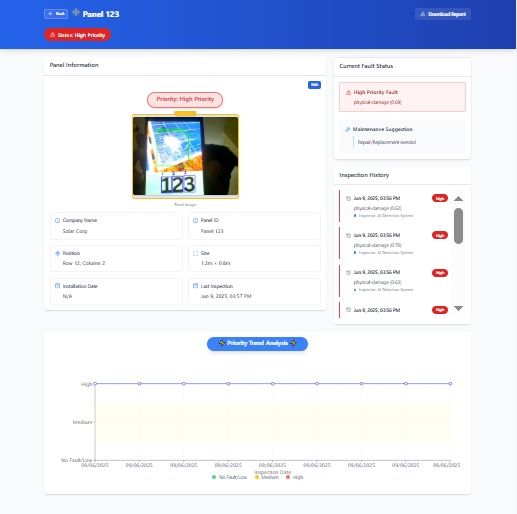
\includegraphics[width=0.75\textwidth]{figure/5.3.jpeg}
\caption{Risk classification of faults}
\label{fig:riskclassification}
\end{figure}

Fig.~\ref{fig:riskclassification} illustrates the categorization of detected faults based on severity and operational impact. Such classification assists maintenance teams in prioritizing repair and inspection activities.

\section{Performance Comparison}

The performance of the proposed system can be evaluated based on parameters such as detection accuracy, precision, recall, F1-score, and operational reliability.

\begin{table}[htb]
\centering
\caption{Performance metrics of the inspection system}
\begin{tabular}{|c|c|c|}
\hline
\textbf{Parameter} & \textbf{Observed Value} & \textbf{Remarks} \\
\hline
Precision & 0.70 & Good detection capability \\
\hline
Recall & 0.60 & Effective fault identification \\
\hline
F1-Score & 0.65 & Balanced performance \\
\hline
mAP@50 & 0.80 & Strong object detection accuracy \\
\hline
System Reliability & High & Stable operation observed \\
\hline
\end{tabular}
\label{tab:performance}
\end{table}

The system demonstrates satisfactory performance for a prototype implementation. Compared to traditional manual inspection techniques, the proposed system significantly improves inspection speed, reduces human effort, and enhances fault detection capability.

\section{Analysis of Results}

The results indicate that the integration of drone-based image acquisition, computer vision, and deep learning has been successfully achieved. The inspection system efficiently captures and processes large volumes of image data while maintaining acceptable detection accuracy.

The RGB analysis module effectively detects defects such as dust accumulation, bird droppings, physical damage, electrical damage, and snow coverage. The trained YOLO model demonstrates reliable object localization and classification performance across multiple inspection scenarios.

The centralized dashboard improves operational awareness by presenting inspection data in an organized and user-friendly format. This allows maintenance teams to prioritize repairs and optimize maintenance schedules.

However, certain limitations were observed. Detection accuracy can be affected by lighting conditions, weather variations, image quality, and dataset diversity. Additionally, certain defect categories with limited training samples may result in occasional misclassifications.

\section{Interpretation of Results}

The experimental outcomes confirm that the system meets its primary objectives of automated inspection, fault detection, and maintenance support. The combination of drone-based image acquisition and deep learning provides an effective approach for monitoring large-scale solar installations.

The use of drone-assisted inspection significantly reduces inspection time while improving coverage of large installations. Deep learning models provide automated fault classification capabilities, reducing dependency on manual inspection processes.

These results indicate that intelligent inspection systems can play an important role in improving the efficiency, reliability, and sustainability of solar energy infrastructure.

\section{Discussion}

The proposed system successfully demonstrates the feasibility of an intelligent drone-assisted inspection framework for solar farms. The modular design allows easy integration of additional technologies and future enhancements.

The current implementation serves as a proof of concept for large-scale renewable energy monitoring systems. By combining aerial inspection, artificial intelligence, and computer vision techniques, the system offers a practical solution for improving maintenance efficiency and reducing operational costs.

Future enhancements may include improved deep learning models, autonomous flight path optimization, larger training datasets, predictive maintenance capabilities, and integration with cloud-based analytics platforms. These improvements can further enhance inspection accuracy and system scalability.

\section{Chapter Summary}

This chapter presented the experimental results and performance analysis of the Visual Inspection of Solar Farm system. The system was found to be effective in detecting solar panel defects and generating maintenance reports through automated analysis. The trained model achieved a Precision of 0.70, Recall of 0.60, F1-Score of approximately 0.65, and mAP@50 of 0.80, validating the effectiveness of the proposed approach. The next chapter concludes the report and outlines future directions for improving the system.

